\chapter{Introduction to Groups}

\section{\textit{Brief} History of Groups}

Back in around 2,000 B.C.---approximately 4,000 years ago---the Babylonians came up with linear and quadratic equations. Specifically, we have equations such as
\[
\begin{aligned}
    ax + b &= 0 \\
    ax^2 + bx + c &= 0
\end{aligned}
\]
We also have the quadratic equation formula:
\[
    x = \frac{-b \pm \sqrt{b^2 - 4ac}}{2a}
\]
Then, in the 1,500s, Cardano, Fontana (or Tartaglia), and Ferro came up with the cubic equations. Specifically, equations in the form
\[
    ax^3 + bx^2 + cx + d = 0
\]
Later on in 1540, Ferrari came up with the quartic equations:
\[
    ax^4 + bx^3 + cx^2 + dx + e = 0
\]
So far, all of these equations have a general solution. That is, we are able to solve these equations in terms of radicals (taking the \(n\)-th roots). Introducing quintic equations:
\[
    ax^5 + bx^4 + cx^3 + dx^2 + ex + f = 0
\]
The (complete version of) Abel-Ruffini theorem from 1824 showed that there is no such general solution just by using the \(+, -, \times, \div, \sqrt[n]{\phantom{(}\cdot\phantom{)}}\) operations.

The concept of \textit{groups} arose from the study of these (and polynomial) equations. Namely, it started from Evariste Galois in the 1830s who used the term group to describe the symmetry of the roots of an equation. This group is now called the \textit{Galois Group}. In general, groups were used to handle mathematical structures in a universal way. Some authors consider it the central organizing principle of contemporary mathematics as it shows up everywhere inside and outside of mathematics.

\section{Symmetry of a Square}

The goal of this section is to identify every possible way that we can remove a square region from a plane and move it in such a way that it can be placed back in the original location. More specifically, we want to describe the relationship between the initial and final positions of this square. For now, we can identify two kinds of movements: rotation and flipping. However, notice that a \(90^\circ\) rotation and a \(450^\circ\) rotation have the same net effect---making them equivalent in this view.

Suppose that we painted a square piece of paper with the colors pink, white, green, and blue. We can now claim that there are exactly 8 ways a square object can be repositioned.

\begin{figure}[ht]
    \centering
    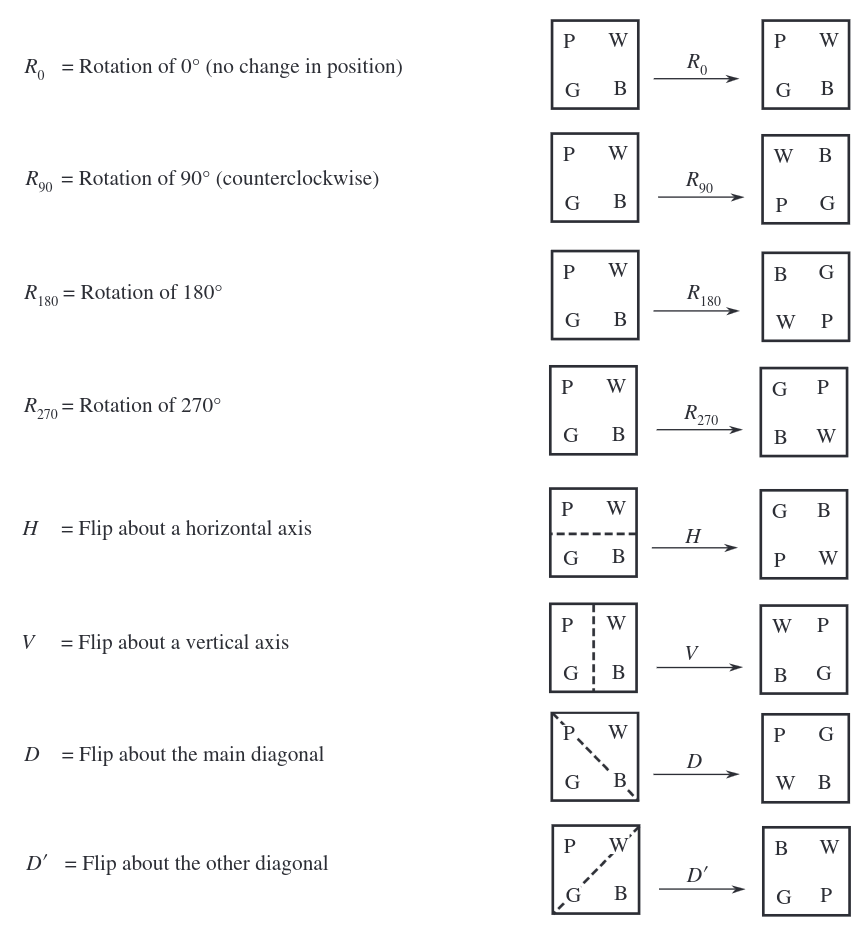
\includegraphics[width=0.65\textwidth]{images/ch1-movements-of-square.png}
    \caption{All possible motions that can be done on a square}
    \label{fig:sqmovements}
\end{figure}

\begin{figure}[ht]
    \centering
    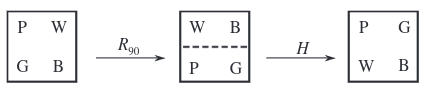
\includegraphics[width=0.6\textwidth]{images/ch1-chain-of-movements.png}
    \caption{Chain of movements being equivalent}
    \label{fig:chainmoves}
\end{figure}

Now, let us investigate some consequences of our claim that any chain of motions is equivalent to a single one from the Figure \ref{fig:sqmovements}. Suppose we rotate once by \(90^\circ\) and then flip along the horizontal axis. Notice in Figure \ref{fig:chainmoves} that this is equivalent to a single flip along the diagonal.

This observation suggests that the 8 motions can be viewed as functions from the square region to itself and we can \textit{compose} them together. Namely, let \(H\) be the horizontal flip, \(R_{d}\) be a clock-wise rotation of \(d\) degrees, and \(D\) be the flip along the main diagonal, we can write the chain of moves previously brought up as follows
\[
    H\ R_{90} = D \text{ or } H \circ R_{90} = D
\]

More generally, the eight motions \(R_0, R_{90}, R_{180}, R_{270}, H, V, D, D'\) together with the operation of composition forms a mathematical structure called the \textit{dihedral group of order 8}, denoted as \(D_4\). Let us now look at some properties of groups by using \(D_4\) as an example.

\section{Properties of Groups}

First, let us construct an \textit{operation table} or a \textit{Cayley table} (named after English mathematician Arthur Caley who introduced them in 1854) for \(D_4\) as follows.

\begin{figure}[ht]
    \centering
    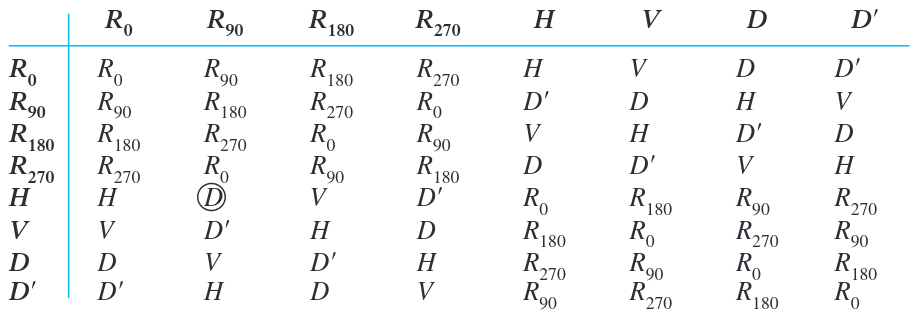
\includegraphics[width=0.8\textwidth]{images/ch1-cayley-table.png}
    \caption{Cayley table for \(D_4\)}
    \label{fig:cayleytable}
\end{figure}

\subsection{Closure}

Notice that the table in Figure \ref{fig:cayleytable} does not introduce any extra motion/element. Algebraically, this means that if elements \(A\) and \(B\) are in \(D_4\), then so is their composition \(AB\). This property is called \textit{closure}.

\subsection{Identity}

Now, notice that the entry of the column for \(R_0\) does not change. That is, if \(A\) is any element of \(D_4\), then \(AR_0 = R_0 A = A\). In this case, the element \(R_0\) is called the identity and every group must have one.

\subsection{Inverse}

Notice also that for every row of the table, there is exactly one corresponding corresponding column whose entry is \(R_0\). Namely, for any element \(A \in D_4\), there is an element \(B \in D_4\) such that \(AB = BA = R_0\). In this case, \(B\) is said to be the inverse of \(A\) and vice versa.

In some cases, an element's inverse is also itself. For example, \(H\) is its own inverse. Intuitively, \(B\) simply undoes what \(A\) does and once these two elements are taken together, they produces the identity element.

\subsection{Associativity}

This condition is something that is quite hard to show for \(D_4\). By itself, associativity of a set is defined by \((ab)c = a(bc)\) where \(a, b,\) and \(c\) are elements of the set. For \(D_4\) specifically, we would need to show this for all \(8^3 = 512\) possible combinations of choices \(a, b, c \in D_4\). However, to make our lives easier, we simply observe that the eight motions/elements are simply functions and the operation is function composition. Then, we can derive the property of associativity from the fact that function composition are associative.

\subsection{Commutativity (Optional)}

Observe that \(HD \neq DH\) but \(R_{90}R_{180} = R_{180}R_{90}\). This means that the order of composition of elements do matter in some cases but not in every group. If a group whose elements \(a, b\) satisfies \(ab = ba\), then we call that group \textit{commutative} or \textit{Abelian} (after the Norwegian mathematician Niels Abel. Otherwise, we say that the group is \textit{non-Abelian}.

\section{The Dihedral Group}

The analysis carried in the previous chapter can be similarly done for any regular/equilateral \(n\)-gon where \(n \geq 3\). The corresponding group is denoted by \(D_n\) and is called the \textit{dihedral group of order \(2n\)}. It is also often called the \textit{group of symmetries of a regular \(n\)-gon}. It has a few properties as follows.

\subsection{Rotational Symmetry}

The \textit{rotational/plane symmetry} of a figure \(F\) in a plane is a function that carries \(F\) onto itself and preserves distance. That is, suppose that \(f: F \to F\) is a function with plane symmetry and points \(p, q \in F\), then \(dist(p, q) = dist(f(p), f(q))\). In addition, the \textit{symmetry group} of a plane is the set of all symmetries of said plane. The definition in 3-D is analogous to this 2-D counterpart.

\subsection{Reflection Symmetry}

The \textit{reflection across a line \(L\)} is the function that leaves every point on \(L\) fixed and sends any point \(q \notin L\) to location \(q'\) such that \(L\) is the perpendicular bisector of the line segment joining \(q\) and \(q'\). The reflection across a plane in 3-D is defined analogously.

A fun observation we can make is that, in order to reflect an object across some point/axis/plane, we need an extra dimension. To illustrate, imagine we want to reflect a piece of paper (a plane in 2D) down its middle, we need to flip it in the third dimension. This means that many objects and figures may have rotational symmetry but not reflective symmetry.
